\documentclass[conference]{IEEEtran}
\IEEEoverridecommandlockouts
% The preceding line is only needed to identify funding in the first footnote. If that is unneeded, please comment it out.
\usepackage{cite}
\usepackage{amsmath,amssymb,amsfonts}
\usepackage{algorithmic}
\usepackage{graphicx}
\usepackage{textcomp}
\usepackage{xcolor}
\def\BibTeX{{\rm B\kern-.05em{\sc i\kern-.025em b}\kern-.08em
    T\kern-.1667em\lower.7ex\hbox{E}\kern-.125emX}}
\begin{document}

\title{Performace on differnet parameter setting in GA-BPNN\\
% {\footnotesize \textsuperscript{*}Note: Sub-titles are not captured in Xplore and should not be used}
% \thanks{Identify applicable funding agency here. If none, delete this.}
}

\author{\IEEEauthorblockN{1\textsuperscript{st} Zih Jie Lin}
\IEEEauthorblockA{\textit{Computer Science Information Engineering.} \\
\textit{Fu Jen Catholoic University}\\
New Taipei City, Taiwan \\
406261597@gapp.fju.edu.tw}
}
% \and
% \IEEEauthorblockN{2\textsuperscript{nd} Given Name Surname}
% \IEEEauthorblockA{\textit{dept. name of organization (of Aff.)} \\
% \textit{name of organization (of Aff.)}\\
% City, Country \\
% email address or ORCID}
% \and
% \IEEEauthorblockN{3\textsuperscript{rd} Given Name Surname}
% \IEEEauthorblockA{\textit{dept. name of organization (of Aff.)} \\
% \textit{name of organization (of Aff.)}\\
% City, Country \\
% email address or ORCID}
% \and
% \IEEEauthorblockN{4\textsuperscript{th} Given Name Surname}
% \IEEEauthorblockA{\textit{dept. name of organization (of Aff.)} \\
% \textit{name of organization (of Aff.)}\\
% City, Country \\
% email address or ORCID}
% \and
% \IEEEauthorblockN{5\textsuperscript{th} Given Name Surname}
% \IEEEauthorblockA{\textit{dept. name of organization (of Aff.)} \\
% \textit{name of organization (of Aff.)}\\
% City, Country \\
% email address or ORCID}
% \and
% \IEEEauthorblockN{6\textsuperscript{th} Given Name Surname}
% \IEEEauthorblockA{\textit{dept. name of organization (of Aff.)} \\
% \textit{name of organization (of Aff.)}\\
% City, Country \\
% email address or ORCID}

\maketitle

\begin{abstract}
GA-BANN is an easy and well-known hybrid network. As the name, the GA-BPNN is what backpropagation neutral network with genetic algorithm searching the parameters. Altough the hybrid network seems to convenient, it's difficult to finds to goood solution beacause the paramerters of backpropagation neutral network is large. This paper design the differnet strategies to run GA-BPNN, and test which performace is better. 
\end{abstract}

\begin{IEEEkeywords}
GA-BPNN, genetic algorithm, backpropagation
\end{IEEEkeywords}

\section{Introduction}
Backpropagation neutral network is a commly neutral network, it can classfiy the model whether is linear. The difficult about backpropagation neutral network is find a parameter set. It's a feasible way to adopt a hybrid model to automatically find solution. A hybrid model is a model combine two or model structure or algorithm. GA-BPNN is the one.\\

GA-BANN is a hybrid network comine with genetic algorithm and backpropagation neutral network. Genetic algorithm uses to evolute paramerters, then apply to backpropagation neutral network. It is to implement. However, due to the range of paremeters is infinity. The accuracy rate of GA-BPNN is often low. To solve this, we use two differnet genetic algorithm to determine whether changing mutation can improve accuracy rate.\\

Genetic algorithm involves population, crossover, mutation. Backpropagation neutral network involves weight, bias, the number of neurons in hidden layer and dropout. The genetic algorithm will adjust weight and bias.\\ 

\subsection{Backpropagation Neutral Network}
Backpropagation Neutral Network is a three-layers neutral network. Fisrt is input layer, second is hidden layer, third is output layer.\cite{b2}\\

\begin{figure}[htbp]
\centerline{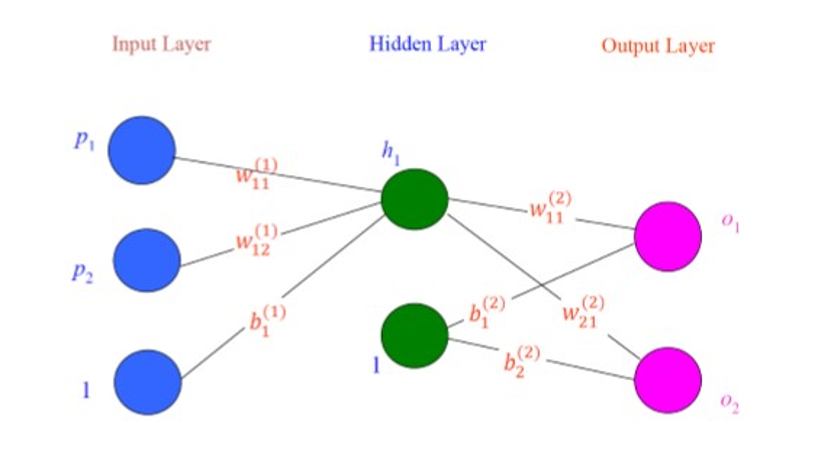
\includegraphics[width=8cm]{Backpropagation.png}}
\caption{Backpropagation Structure}
\label{fig}
\end{figure}

It uses gradient descent to adjust weight and bias.\\

\begin{equation}
\label{gradient_descent}
\nabla f(x, y) = \left[
\begin{array}{ccc}
\frac{\partial f(x, y)}{\partial x}\\
\frac{\partial f(x, y)}{\partial y}\\
\end{array}
\right]
\end{equation}

The activation function we choose is:\\

\begin{equation}
\label{activation_function}
a(n)=\frac{1}{1+e^{-n}}
\end{equation}

\begin{equation}
\label{activation_function_2}
\frac{da(n)}{dn}=a(1-a)
\end{equation}
	
The loss function is:\\

\begin{equation}
\label{loss_function}
E(a)=(t-a)^2
\end{equation}

\begin{equation}
\label{loss_function_2}
\frac{dE(a)}{da}=-2(t-a)
\end{equation}

The following is the process of calculating backpropogation basd on above 4 equations:\\

First calculate output of hidden layer and output layer forward:\\

\begin{equation}
\label{hidden_layer_output}
a_{h1}=\sigma(W^{(1)}p+b^{(1)})
\end{equation}

\begin{equation}
\label{output_layer_output}
a=\sigma(W^{(2)}a_{h1}+b^{(2)})
\end{equation}

Then calculate error backward base on output $a$ and target output $t$:\\

\begin{equation}
\label{output_layer_error}
\delta=(t-a)[a(1-a)]
\end{equation}

\begin{equation}
\label{hidden_layer_error}
\delta_{h1}=(W^{(2)}\delta)[a_{h1}(1-a_{h1})]
\end{equation}

Finally, update the update:\\

\begin{equation}
\label{output_layer_update_weight}
W^{(2)}=W^{(2)} + 2\alpha\delta a_{h1}
\end{equation}

\begin{equation}
\label{output_layer_update_bias}
b^{(2)}=b^{(2)} + 2\alpha\delta
\end{equation}

\begin{equation}
\label{hidden_layer_update_weight}
W^{(1)}=W^{(1)} + 2\alpha\delta_{h1}p
\end{equation}

\begin{equation}
\label{hidden_layer_update_bias}
b^{(1)}=b^{(1)} + 2\alpha\delta_{h1}
\end{equation}

$\alpha$ is learning rate, the update range. It's often a small value at the end of process in order to easliy find the optimal solution.\\

\subsection{Genetic algorithm}
Genetic algorithm is a method inspired by the natural process. The process can be divide into 6 parts.\\

First is generating population the process will generate $L$ population.\\

Second part is evaluate the every poppulation's fitness, the fitness can be defined widely. In GA-BPNN, we can defined the the accuracy rate of testing data.\\

Third is parent selection, we use 2-tournament selection, that is, select 2 parents randomly and retain the one has higher fitness.\\

The fourth step is crossover. We define a constant, $p_c$, is the rate of crossover, and use random function as roulette. When the result of roulette is $< p_c$ do crossover, otherwise not to do.\\

After crossover is mutation, like crossover, $p_m$ is the 
rate of mutation.\\

Final is surival selection, select best $L$ population from parents or offspring based on fitness. That's the whole process of genetic algorithm.\cite{b1}\\

\begin{figure}[htbp]
\centerline{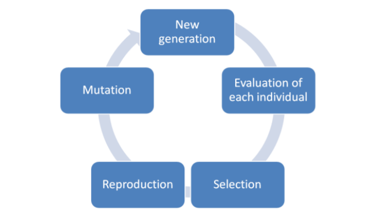
\includegraphics[width=8cm]{Genetic_algorithm.png}}
\caption{Process of Genetic Algorithm}
\label{fig}
\end{figure}


\subsection{Structute of GA-BPNN}
In the genetic algorithm, every individual has own chromosome (parameter set). When the chrmosome changes (like mutation), the genetic algorithm need to call backpropagation neutral network to evulate fitness.

\begin{figure}[htbp]
\centerline{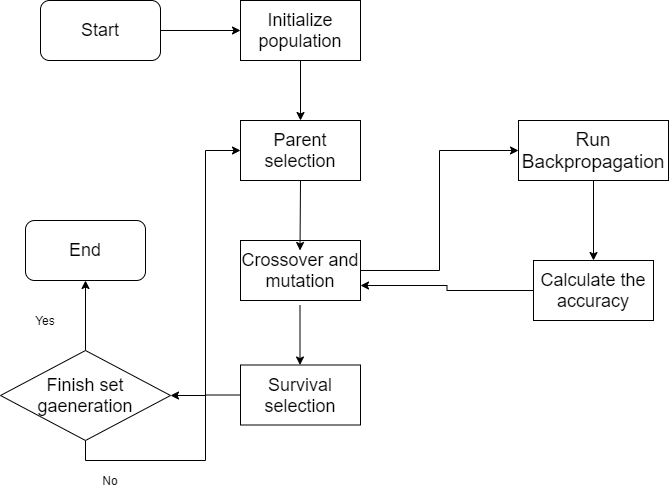
\includegraphics[width=8cm]{BP_GANN_structure.png}}
\caption{BP-GANN structure}
\label{fig}
\end{figure}

\section{Data and result analysis}
\subsection{Data}
The iris dataset has 150 items. Input has 4 features, sepal length, sepal width, petal length and petal width. Output is the species name: setosa, virginica and versicolor.

\begin{table}[htbp]
\caption{Dataset sample}
\begin{center}
\begin{tabular}{|c|c|c|c|c|}
\hline
Sepal length & Sepal width & Petal length & Petal width & Output \\
\hline
6 & 2.7 & 5.1 & 1.6 & versicolor \\
\hline
7.1 & 3 & 5.9 & 2.1 & virginica \\
\hline
5.4 & 3.4 & 1.7 & 0.2 & setosa \\
\hline
5.8 & 2.7 & 5.1 & 1.9 & virginica \\
\hline
6.7 & 3 & 5.2 & 2.3 & virginica \\
\hline
6.7 & 3 & 5 & 1.7 & versicolor \\
\hline
4.8 & 3.1 & 1.6 & 0.2 & setosa \\
\hline
4.8 & 3.4 & 1.9 & 0.2 & setosa \\
\hline
5.6 & 2.7 & 4.2 & 1.3 & versicolor \\
\hline
\end{tabular}
\label{dataset_sample}
\end{center}
\end{table}

\subsection{Design}
\begin{itemize}
\item Dimension: 11. Include the value of $W^{(1)}, b^{(1)}, W^{(2)}, b^{(2)}$
\item Fitness: accuracy rate of testing Data, accuracy rate of training Data
\item Population size = 40
\item Generation = 100
\item Crossover Rate = 0.9
\end{itemize}

The expriment has two version. Version 1 is the mutation rate of all chromosome is $0.1$. Version 2 is the mutation rate of initial $W^{(1)}, b^{(1)}$ all chromosome is $0.2$, the mutation rate of initial $W^{(2)}, b^{(2)}$ all chromosome is $0.05$. The intention of version 2 is test whether the initial weight and bias in input layer is more important than the initial weight and bias in hidden layer.\\

\subsection{Result}
The experiment is excuted in GNU G++. Each version is excuted 30 times. The charts below respectively represent version 1 and version 2, is the average accuracy rate of testing data.\\

\begin{figure}[htbp]
\centerline{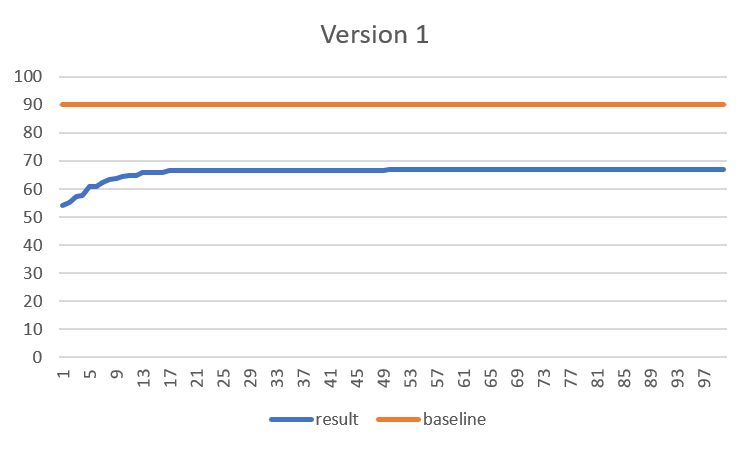
\includegraphics[width=8cm]{version1.png}}
\caption{Accuracy rate of testing data in version 1}
\label{fig}
\end{figure}

\begin{figure}[htbp]
\centerline{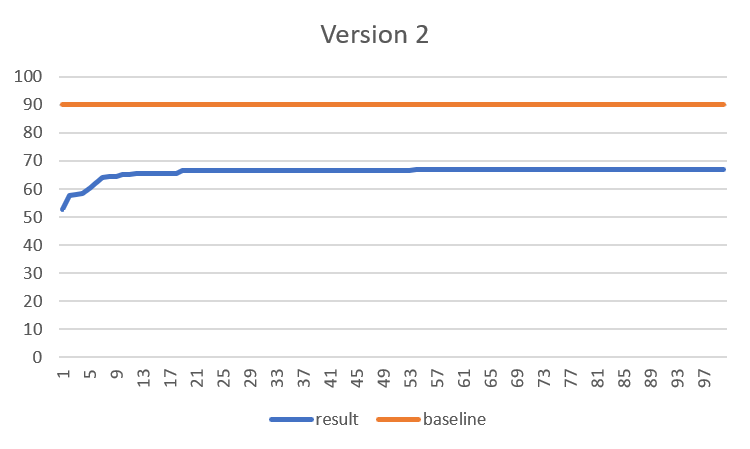
\includegraphics[width=8cm]{version2.png}}
\caption{Accuracy rate of testing data in version 2}
\label{fig}
\end{figure}

The result show that there's no obvious difference between two version. The final accuracy rate of testing data is near 70\% which is far away the baseline 90\%. Both of them converge around twentieth generation.

\section{Conclusion}
In the paper, we introduce GA-BPNN and point out it's disadvantage, it hardly to find a proper solution. Then we propose two different method to determine the accuracy can improve. After experiment done, we make a conclusion that it's useless to adjust mutation rate. We need to change the strategy. One way is adjust the crossover rate or mutation rate basd on change of fitness. Another way is revise chromosome. Chromosome can be the structure of backpropagation neutral network, like dropout or number of neuron.

\begin{thebibliography}{00}
\bibitem{b1} Li Jiacheng and Li Lei
, A Hybrid Genetic Algorithm Based on Information Entropy and Game Theory, IEEEAccess Volume 8, 2020
\bibitem{b2} Martin T. Hagan Oklahoma State University Stillwater, Oklahoma Howard B. Demuth University of Colorado Boulder, Colorado Mark Hudson Beale MHB Inc. Hayden, Idaho Orlando De Jesús Consultant Frisco, Texas, Neural Network Design 2nd Edtion 

\end{thebibliography}
\vspace{12pt}

\end{document}
